\documentclass[11pt]{article}

\usepackage[margin=1in]{geometry}
\usepackage{booktabs}
\usepackage{array}
\usepackage{enumitem}
\usepackage{float}
\usepackage{graphicx}
\usepackage{amsmath}
\usepackage{amssymb}
\usepackage[hidelinks,pdfborder={0 0 0}]{hyperref}
\usepackage{tikz}
\usetikzlibrary{arrows.meta,positioning,calc,fit,backgrounds}

\newcommand{\code}[1]{\texttt{\detokenize{#1}}}
\newcommand{\pct}[1]{#1\%}
\newcommand{\loss}{\mathcal{L}}

\title{Interim Report: May 2026 PA-CSI DG Experiments}
\author{Zihao Wang}
\date{May 2026}

\begin{document}
\maketitle

\section{Progress: May Experiments and Results}

\subsection{Reference Line, Not a May Attempt}

The April paper-aligned SupCon result remains the most important reference for judging new experiments. It is included here only to define the comparison target:
\[
\text{SupCon reference: mean LOEO accuracy}=90.27\%,\qquad
\text{mean macro-F1}=88.20\%.
\]
This reference covers $E1$, $E2$, and $E3$ with seed 42. It should not be described as a new May experiment. The May experiments below are attempts to improve the geometry of the contrastive representation and the local class boundaries.

\subsection{Sub-center Prototype SupCon}

The first May direction was to replace pairwise SupCon geometry with class prototypes. Instead of pulling all same-class embeddings toward one implicit class cluster, each class owns $K$ learnable sub-centers. This is intended to match the multi-mode structure of PA-CSI data, where the same activity can appear differently under different environments, body orientations, and antenna-view responses.

\begin{table}[H]
\centering
\small
\caption{May sub-center prototype screening on target $E2$, seed 42.}
\label{tab:subcenter_screen}
\resizebox{\textwidth}{!}{%
\begin{tabular}{p{2.0in}cccccp{1.55in}}
\toprule
Experiment & Epochs & $K$ & PairMargin & Acc. & Macro-F1 & Observation \\
\midrule
Sub-center prototype, layer 1 & 40 & 2 & off & 88.17 & 86.08 & Strong without pair margin \\
Sub-center prototype, layer 1 & 40 & 2 & on & 87.17 & 85.40 & Margin did not help at $K=2$ \\
Sub-center prototype, layer 1 & 40 & 3 & off & 86.30 & 83.51 & More centers alone was unstable \\
Sub-center prototype, layer 1 & 40 & 3 & on & 88.73 & 86.73 & Best layer-1 screening result \\
Sub-center prototype, layer 2 & 200 & 3 & on & \textbf{90.23} & \textbf{88.24} & Best May result so far \\
Sub-center prototype, layer 2 & 200 & 5 & on, $0{\rightarrow}4$ & 88.73 & 86.11 & More centers did not improve $E2$ \\
\bottomrule
\end{tabular}
}%
\end{table}

The key outcome is that $K=3$ with fixed PairMargin became the best May setting on $E2$. The result is close to the April full-LOEO SupCon reference and slightly stronger than the reference's $E2$ result, but it is not yet a complete full-LOEO conclusion because it has not been verified across $E1$ and $E3$ under the same final setting.

\subsection{K and Margin Search}

The second May direction was to search the margin design more systematically. The search covered $K=4$ and $K=5$, no-margin references, raw shared margins, raw pair-specific margins, and quantile pair-specific margins. The repeated hard pairs were:
\[
0{\rightarrow}4,\qquad 1{\rightarrow}4,\qquad 4{\rightarrow}1.
\]
The search generated source-validation and target-test diagnostics including confusion matrices, gap statistics, margin violation statistics, prototype occupancy, and effective prototype usage.

\begin{table}[H]
\centering
\small
\caption{Source-validation selected candidates from the K/margin search.}
\label{tab:kmargin_candidates}
\resizebox{\textwidth}{!}{%
\begin{tabular}{clp{3.65in}}
\toprule
Target & Selected candidates & Interpretation \\
\midrule
$E1$ & $K=5$, raw pair-specific $0{\rightarrow}4$ with $m=0.00$ or $m=0.15$ & The search suggested that $E1$ may prefer a larger prototype bank and a local correction around class 0 versus class 4. \\
$E2$ & $K=4$, raw pair-specific $0{\rightarrow}4$ with $m=0.20$, or quantile $0{\rightarrow}4$ with $q=0.10$ & The $E2$ result again points to local pair-specific boundaries rather than a global margin. \\
$E3$ & $K=4$, quantile $1{\rightarrow}4$ with $q=0.10$, or raw pair-specific $4{\rightarrow}1$ with $m=0.20$ & The selected pair changes by target, which is evidence that hand-selected margins may not transfer cleanly. \\
\bottomrule
\end{tabular}
}%
\end{table}

The important lesson is that local margins are useful, but the best pair and best value are not stable across targets. This directly motivates the later dynamic margin and LCA-KM attempts.

\subsection{Dynamic Pair Margin}

The third May direction was to update PairMargin values during training instead of keeping them fixed. After a warm-up period, the method estimates the source-validation gap for each candidate pair, clips it into a valid margin range, and applies an exponential moving average. This was implemented for the sub-center prototype loss and tested on $E2$.

\begin{table}[H]
\centering
\small
\caption{Dynamic pair-margin experiments on target $E2$, seed 42.}
\label{tab:dynamic_margin}
\resizebox{\textwidth}{!}{%
\begin{tabular}{p{3.3in}ccccl}
\toprule
Experiment & Epochs & $K$ & Acc. & Macro-F1 & Observation \\
\midrule
Dynamic PairMargin smoke run & 30 & 3 & 87.77 & 85.36 & Implementation and artifact path verified \\
Dynamic PairMargin full run & 200 & 3 & 87.53 & 84.91 & Stable but below the fixed $K=3$ PairMargin run \\
\bottomrule
\end{tabular}
}%
\end{table}

The dynamic version is useful as a mechanism, but its current result is weaker than the fixed margin run. This suggests that simply estimating a quantile gap and smoothing it is not enough; the pair selection and margin objective must be better aligned with source-domain hardness.

\subsection{LCA-KM: LOSO-Calibrated Adaptive K-Margin}

The fourth May direction was LCA-KM. This method tries to remove manual pair selection by recalibrating hard negative pairs from source data only. For each source environment, it builds leave-one-source-out class prototypes from the other source environments, evaluates class-pair hardness on the held-out source environment, and selects an adaptive number of negative class pairs per class. The target environment is not used for calibration.

\begin{table}[H]
\centering
\small
\caption{Adaptive K-margin experiments available in the current workspace.}
\label{tab:lcakm}
\resizebox{\textwidth}{!}{%
\begin{tabular}{p{3.15in}cccp{1.8in}}
\toprule
Experiment & Target / scope & Acc. & Macro-F1 & Observation \\
\midrule
LCA-KM smoke verify & $E2$ & 73.93 & 69.39 & Smoke-level verification only \\
Mini-validation SupCon reference & $E2$ & 74.27 & 70.21 & Small validation setup, not canonical \\
Mini-validation LCA-KM & $E2$ & 74.40 & 70.00 & Similar to mini-validation reference \\
LCA-KM base & $E3$ & 83.80 & 81.73 & Source-calibrated method runs end to end \\
Paper-aligned LCA-KM retry & $E2$ & 89.80 & 87.65 & Stronger configuration, close to reference but below fixed $K=3$ PairMargin \\
\bottomrule
\end{tabular}
}%
\end{table}

At this stage, LCA-KM is more important as a research direction than as the best result. It is a source-only way to discover hard negative pairs, which is exactly what is needed if the final method should work on future datasets instead of relying on the known confusions of this dataset.

\section{Why I Use These Methods}

\subsection{The Representation Problem}

For each PA-CSI sample $x_i$, the model produces a normalized projection embedding
\[
z_i = \frac{g_\phi(f_\theta(x_i))}{\|g_\phi(f_\theta(x_i))\|_2},
\qquad
y_i \in \{1,\dots,C\}.
\]
The domain-generalization goal is not only to classify the source environments, but to learn a geometry where samples from unseen environments remain close to the correct activity class. In PA-CSI, the same class can be multi-modal because CSI depends on body orientation, location, propagation path, and antenna response. Therefore, one class should not necessarily be forced into one compact point.

\begin{figure}[H]
\centering
\resizebox{\textwidth}{!}{%
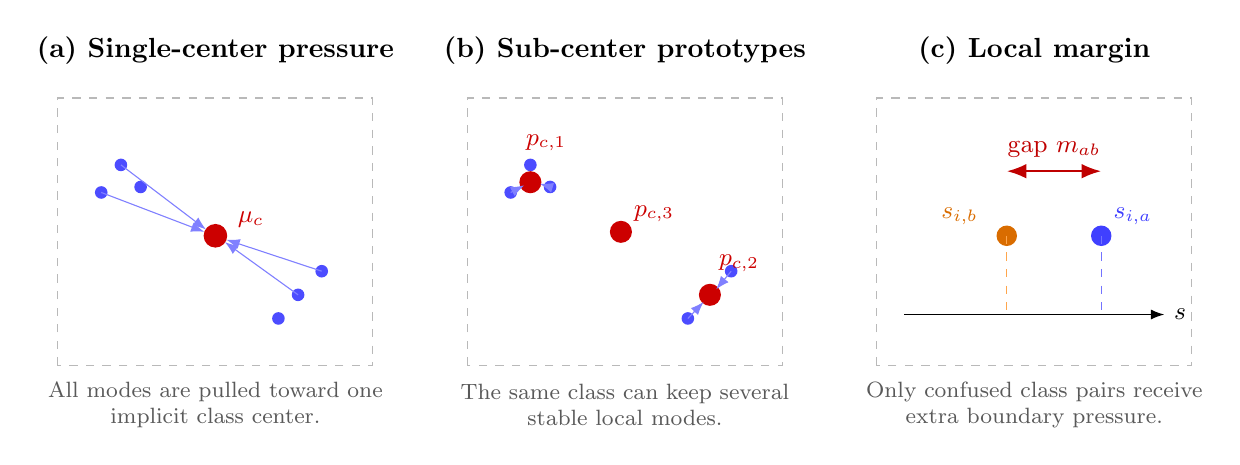
\begin{tikzpicture}[font=\small, >=Latex]
% Panel A
\begin{scope}[shift={(0,0)}]
  \node[font=\bfseries] at (0,2.35) {(a) Single-center pressure};
  \draw[gray!55, dashed] (-2.0,-1.65) rectangle (2.0,1.75);
  \fill[blue!70] (-1.2, 0.9) circle (0.08);
  \fill[blue!70] (-1.45, 0.55) circle (0.08);
  \fill[blue!70] (-0.95, 0.62) circle (0.08);
  \fill[blue!70] (1.05,-0.75) circle (0.08);
  \fill[blue!70] (1.35,-0.45) circle (0.08);
  \fill[blue!70] (0.80,-1.05) circle (0.08);
  \fill[red!80!black] (0,0) circle (0.15);
  \node[red!80!black] at (0.45,0.2) {$\mu_c$};
  \draw[->, blue!50] (-1.2,0.9) -- (-0.12,0.08);
  \draw[->, blue!50] (-1.45,0.55) -- (-0.14,0.05);
  \draw[->, blue!50] (1.05,-0.75) -- (0.12,-0.08);
  \draw[->, blue!50] (1.35,-0.45) -- (0.14,-0.05);
  \node[align=center, font=\footnotesize, text=black!65] at (0,-2.15)
    {All modes are pulled toward one\\implicit class center.};
\end{scope}

% Panel B
\begin{scope}[shift={(5.2,0)}]
  \node[font=\bfseries] at (0,2.35) {(b) Sub-center prototypes};
  \draw[gray!55, dashed] (-2.0,-1.65) rectangle (2.0,1.75);
  \fill[blue!70] (-1.2, 0.9) circle (0.08);
  \fill[blue!70] (-1.45, 0.55) circle (0.08);
  \fill[blue!70] (-0.95, 0.62) circle (0.08);
  \fill[blue!70] (1.05,-0.75) circle (0.08);
  \fill[blue!70] (1.35,-0.45) circle (0.08);
  \fill[blue!70] (0.80,-1.05) circle (0.08);
  \fill[blue!70] (-0.05,0.05) circle (0.08);
  \fill[red!80!black] (-1.2,0.68) circle (0.14);
  \fill[red!80!black] (1.08,-0.75) circle (0.14);
  \fill[red!80!black] (-0.05,0.05) circle (0.14);
  \node[red!80!black] at (-1.0,1.18) {$p_{c,1}$};
  \node[red!80!black] at (1.45,-0.35) {$p_{c,2}$};
  \node[red!80!black] at (0.37,0.28) {$p_{c,3}$};
  \draw[->, blue!50] (-1.45,0.55) -- (-1.28,0.64);
  \draw[->, blue!50] (-0.95,0.62) -- (-1.08,0.66);
  \draw[->, blue!50] (1.35,-0.45) -- (1.16,-0.68);
  \draw[->, blue!50] (0.80,-1.05) -- (1.00,-0.84);
  \node[align=center, font=\footnotesize, text=black!65] at (0,-2.15)
    {The same class can keep several\\stable local modes.};
\end{scope}

% Panel C
\begin{scope}[shift={(10.4,0)}]
  \node[font=\bfseries] at (0,2.35) {(c) Local margin};
  \draw[gray!55, dashed] (-2.0,-1.65) rectangle (2.0,1.75);
  \draw[->] (-1.65,-1.0) -- (1.65,-1.0) node[right] {$s$};
  \fill[orange!85!black] (-0.35,0.0) circle (0.13);
  \node[orange!85!black] at (-0.95,0.25) {$s_{i,b}$};
  \draw[orange!70, dashed] (-0.35,0) -- (-0.35,-1.0);
  \fill[blue!75] (0.85,0.0) circle (0.13);
  \node[blue!75] at (1.25,0.25) {$s_{i,a}$};
  \draw[blue!55, dashed] (0.85,0) -- (0.85,-1.0);
  \draw[<->, red!75!black, line width=0.9pt] (-0.35,0.82) -- (0.85,0.82);
  \node[red!75!black] at (0.25,1.1) {gap $m_{ab}$};
  \node[align=center, font=\footnotesize, text=black!65] at (0,-2.15)
    {Only confused class pairs receive\\extra boundary pressure.};
\end{scope}
\end{tikzpicture}%
}
\caption{Why the May methods focus on prototype geometry and local margins. (a) A single-center pressure can collapse multi-mode PA-CSI activity structure. (b) Sub-center prototypes allow several modes per class. (c) Directed PairMargin focuses on local confused class pairs instead of increasing global contrastive pressure for all negatives.}
\label{fig:geometry}
\end{figure}

\subsection{Why Sub-center Prototype SupCon}

Let $p_{c,k}$ be the $k$-th normalized prototype of class $c$, where $k=1,\dots,K$. The score between sample $i$ and class $c$ is the best sub-center similarity:
\[
s_{i,c} = \max_{1\le k\le K} z_i^\top p_{c,k}.
\]
The prototype contrastive loss can be written as
\[
\loss_{\mathrm{proto}}(i)
=
-\log
\frac{\exp(s_{i,y_i}/\tau)}
{\sum_{c=1}^{C}\sum_{k=1}^{K}\exp(z_i^\top p_{c,k}/\tau)}.
\]
The numerator says that the sample only needs to match one good mode of its true class. The denominator still compares against all class sub-centers, so different classes remain separated. This is why I use sub-center prototypes: the method preserves multimodal intra-class structure while still creating cross-class repulsion.

\paragraph{How I search $K$ for this method.}
Here $K$ is a model-capacity parameter, not just a tuning detail. With $C$ classes and embedding dimension $d$, the prototype table has $C K d$ parameters and the contrastive denominator has $C K$ prototype terms. If $K$ is too small, several physical CSI modes of the same activity must share one prototype. If $K$ is too large, the extra centers can model source-domain noise instead of reusable activity structure.

The search therefore starts by isolating prototype capacity from PairMargin:
\[
K \in \{1,2,3,4,5\},\qquad \lambda_{\mathrm{pair}}=0.
\]
For each held-out target environment $e$ and seed, I train with target $e$ excluded and select $K$ by source-validation macro-F1:
\[
K^\star
=
\arg\max_{K}
\operatorname{MacroF1}_{\mathrm{source\;val}}(K).
\]
The held-out target result is recorded only after selection. In the current May path, $K=3$ became the anchor from the $E2$ layer-1/layer-2 screening, while $K=4$ and $K=5$ are capacity checks around that anchor.

\subsection{Why Directed PairMargin}

The May diagnostics show that the remaining errors are not evenly spread over all negative pairs. They are concentrated in a few directed confusions such as $0{\rightarrow}4$, $1{\rightarrow}4$, and $4{\rightarrow}1$. For a directed pair $(a,b)$, define the similarity gap
\[
g_i^{a,b}=s_{i,a}-s_{i,b},\qquad y_i=a.
\]
The directed PairMargin term is
\[
\loss_{\mathrm{pair}}(i;a,b)
=
\left[m_{a,b}-g_i^{a,b}\right]_+
=
\left[m_{a,b}+s_{i,b}-s_{i,a}\right]_+.
\]
This hinge activates only when the true class score does not exceed the confused negative class score by at least $m_{a,b}$. This is a local boundary correction. It is more targeted than simply increasing the SupCon weight, because it does not force all negative pairs to receive the same additional pressure.

\paragraph{How I search fixed PairMargin.}
For fixed PairMargin, the search has two parts: choose the directed pair and choose the margin value. I start from focus pairs identified by source-side and diagnostic confusion behavior:
\[
\mathcal{P}_{\mathrm{focus}}=\{(1,4),(4,1),(0,4)\}.
\]
For raw margins, I use the grid
\[
m\in\{0.00,0.05,0.10,0.15,0.20\}.
\]
I test both a shared setting, where the same $m$ is applied to all focus pairs, and a pair-specific setting, where only one directed pair receives the margin. The selection criterion is source-validation macro-F1:
\[
(a^\star,b^\star,m^\star)
=
\arg\max_{(a,b)\in\mathcal{P}_{\mathrm{focus}},\,m}
\operatorname{MacroF1}_{\mathrm{source\;val}}(a,b,m).
\]
I also record source-validation violation rate and average hinge shortfall to understand whether a margin is actually active, but target-test accuracy is used only after the source-side choice is made.

For quantile margins, I first run a no-margin model and measure source-validation gaps:
\[
\mathcal{G}_{a,b}
=
\{s_{i,a}-s_{i,b}: y_i=a,\; i\in\text{source validation}\}.
\]
Then the margin is chosen from the pair's own gap distribution:
\[
m_{a,b}(q)=Q_q(\mathcal{G}_{a,b}),\qquad
q\in\{0.10,0.20,\dots,0.80\}.
\]
This is searched as both shared-$q$ and pair-specific-$q$ configurations. The short runs create a source-validation shortlist, and the top configurations are then confirmed with longer 200-epoch runs.

\subsection{Why Dynamic Margin}

Fixed margins can work well on a known target, but they are manually chosen. To reduce hand tuning, the dynamic margin variant estimates the margin from source-validation gaps. For pair $(a,b)$ at recalibration step $t$, let
\[
\mathcal{G}_{a,b}^{(t)}
=
\{s_{i,a}-s_{i,b}: y_i=a,\; i \in \text{source validation}\}.
\]
The raw margin is a clipped low quantile of the gap distribution:
\[
\widehat{m}_{a,b}^{(t)}
=
\operatorname{clip}
\left(
Q_q(\mathcal{G}_{a,b}^{(t)}),
m_{\min},
m_{\max}
\right).
\]
The updated margin is smoothed:
\[
m_{a,b}^{(t)}
=
\beta m_{a,b}^{(t-1)}
+
(1-\beta)\widehat{m}_{a,b}^{(t)},
\]
with an additional maximum step-size constraint. The reason for trying this method is that the margin should reflect the current representation geometry. The current result shows that the mechanism runs, but the simple quantile rule is weaker than the fixed margin, so it needs better pair selection and stability control.

\paragraph{How I search margins in this method.}
Dynamic PairMargin does not search a static grid. I fix the prototype count to the current anchor $K=3$, start from the focus candidate pairs, and let the margin values be recalibrated during training. In the current configuration, recalibration starts after 20 warm-up epochs and repeats every 10 epochs. For each candidate pair, the source-validation gaps are collected and the raw margin is
\[
\widehat{m}_{a,b}
=
\operatorname{clip}
\left(
Q_{0.15}(\mathcal{G}_{a,b}),
0.03,
0.18
\right).
\]
The actual margin used by the loss is smoothed by EMA:
\[
m_{a,b}^{(t)}
=
0.8\,m_{a,b}^{(t-1)}
+
0.2\,\widehat{m}_{a,b},
\]
with a maximum update size of $0.03$ and a minimum class-pair sample count requirement. This means the method searches the margin online from source-validation geometry instead of picking one fixed margin before training.

\subsection{Why LCA-KM}

The most general May idea is LCA-KM, because it avoids target-specific pair selection. Suppose the available source environments are $\mathcal{E}_s$. For each held-out source environment $e\in\mathcal{E}_s$, class prototypes are built from the other source environments:
\[
\mu_c^{(-e)}
=
\frac{
\sum_{i:y_i=c,\;d_i\neq e} z_i
}{
\left\|
\sum_{i:y_i=c,\;d_i\neq e} z_i
\right\|_2
}.
\]
The held-out source environment is then used as a calibration environment. For true class $a$ and negative class $b$, the method estimates four quantities:
\begin{align*}
h_{a,b} &= \text{hardness},\\
v_{a,b} &= \Pr[s_{i,a}-s_{i,b}\le \tau_g],\\
u_{a,b} &= \text{cross-source instability},\\
\kappa_a &= \text{class compactness}.
\end{align*}
In the implementation, hardness is estimated with a softmax over negative class similarities:
\[
h_{a,b}^{(e)}
=
\mathbb{E}_{i:y_i=a,d_i=e}
\left[
\frac{\exp(\beta_s s_{i,b})}
{\sum_{c\neq a}\exp(\beta_s s_{i,c})}
\right].
\]
Violation rate is the fraction of held-out source samples whose true-vs-negative gap is too small:
\[
v_{a,b}^{(e)}
=
\Pr_{i:y_i=a,d_i=e}
\left[
s_{i,a}-s_{i,b}\le \tau_g
\right].
\]
Instability $u_{a,b}$ is the cross-source variation of hardness. After normalization, the pair score is
\[
R_{a,b}
=
\widetilde{h}_{a,b}
\cdot
\widetilde{v}_{a,b}
\cdot
(1-\widetilde{u}_{a,b})
\cdot
\widetilde{\kappa}_a.
\]
The adaptive margin is then
\[
m_{a,b}
=
m_{\min}
+
(m_{\max}-m_{\min})
\sigma(
\alpha\widetilde{h}_{a,b}
+
\beta\widetilde{v}_{a,b}
+
\gamma\widetilde{\kappa}_a
-
\delta\widetilde{u}_{a,b}
).
\]
For each class $a$, LCA-KM ranks negative classes by $R_{a,b}$ and chooses the smallest top set whose cumulative score mass reaches an adaptive threshold $\rho_a$.

\paragraph{How I search pairs, weights, and margins in this method.}
LCA-KM has no manually fixed focus-pair list. After warm-up, it evaluates all valid source class pairs, ranks them by $R_{a,b}$, and selects
\[
S_a
=
\left\{
\text{top-ranked } b
\text{ until cumulative normalized } R_{a,b} \ge \rho_a
\right\}.
\]
The threshold $\rho_a$ is itself adaptive: it increases with source hardness entropy and decreases with cross-source instability. Pair weights are normalized selected scores,
\[
w_{a,b}
=
\frac{R_{a,b}}{\sum_{j\in S_a}R_{a,j}},
\qquad b\in S_a,
\]
and each selected pair uses the adaptive margin $m_{a,b}$ above. Thus LCA-KM searches three things from source calibration at the same time: which negative pairs to use, how many pairs each class needs, and how strong each pair margin should be. The final loss is
\[
\loss_{\mathrm{AKM}}(i)
=
\sum_{b\in S_{y_i}}
w_{y_i,b}
\left[
m_{y_i,b}
-
(s_{i,y_i}-s_{i,b})
\right]_+.
\]
This is the most important mathematical direction for future generalization. It uses only source-domain calibration, it can discover the hard pairs automatically, and it can adapt the number of negative pairs per class. If improved, it is more likely to transfer to future datasets than a manually chosen pair list.

\section{Next Steps}

\begin{enumerate}[leftmargin=*]
    \item \textbf{Keep the current best May method as the anchor.} I will continue with the $K=3$ sub-center prototype SupCon plus directed PairMargin setting, because it is the best May result so far on $E2$ with $90.23\%$ accuracy and $88.24\%$ macro-F1.

    \item \textbf{Verify whether the result is target-specific.} The current best run is not enough by itself because it is focused on $E2$. The next necessary experiment is full LOEO with the same method on $E1$, $E2$, and $E3$, followed by multi-seed validation if the result remains positive.

    \item \textbf{Separate the source of improvement.} I need to compare four controlled variants: pairwise SupCon, sub-center prototype without PairMargin, fixed PairMargin, and adaptive/source-calibrated PairMargin. This will show whether the gain comes from the multi-center geometry, the local margin, or their interaction.

    \item \textbf{Make the margin method less dataset-specific.} The K/margin search shows that the best pair can change by target. For future datasets, I should not rely on manually naming pairs such as $0{\rightarrow}4$ or $1{\rightarrow}4$. The direction should be source-only pair discovery, using LCA-KM or a simpler calibrated hard-pair selector.

    \item \textbf{Test for future-dataset suitability.} The long-term goal is not only to fit this PA-CSI MultiEnv dataset. I will evaluate whether the method can be defined using only information that would exist on a future dataset: source domains, source labels, class prototypes, source-validation gaps, and source-only calibration statistics. A method that needs target-environment confusion knowledge should be treated as a diagnostic tool, not the final general solution.

    \item \textbf{Define the success criterion.} The method should be judged by full-LOEO mean accuracy and macro-F1, per-class stability, multi-seed variance, and whether the same calibration rule works without target-specific manual pair choices. If the fixed PairMargin remains strongest but does not transfer, I will keep it as evidence for the geometry problem and focus the final method on adaptive source-calibrated margins.
\end{enumerate}

\section{Current Conclusion}

The May work has moved from simply adding more global regularization to designing a better contrastive geometry. The current evidence supports three conclusions. First, PA-CSI classes are better modeled with multi-center geometry than with a single implicit class cluster. Second, the hardest errors are local and directed, so a pair-specific margin is more appropriate than a uniform negative pressure. Third, a final publishable method should not depend on hand-picked pairs from this dataset. I will therefore keep the current best $K=3$ sub-center PairMargin method as the experimental anchor, while pushing the next stage toward source-only adaptive calibration that can apply to future datasets.

\vfill
\begin{center}
End of Report
\end{center}

\end{document}
